\documentclass[conference]{IEEEtran}
\usepackage[utf8]{inputenc}
\usepackage[T1]{fontenc}
\usepackage{microtype}
\usepackage{booktabs}
\usepackage{upquote}
\usepackage{graphicx}
\usepackage{color}
\usepackage[hyphens]{url}
\usepackage[colorlinks=true,citecolor=darkgreen]{hyperref}
\usepackage{flushend}

\pdfmapfile{+ttfonts.pdfmap}
\hyphenation{brow-ser brow-sers tra-di-tion-al ja-va-script Web-Kit}
\definecolor{darkgreen}{rgb}{0,0.5,0}

\newcommand*{\lcd}[1]{\hbox{\usefont{T1}{lcd7}{m}{n} #1}}
\newcommand*{\subtitle}[1]{\\\vspace{-0.2em}{\Large\itshape #1}\vspace{0.2em}}

% Formatting adjustments for the bibliography.
\makeatletter
\newcommand*{\BIBdecl}{%
  % Prevent bibliography entries from being split across pages.
  % This is not just cosmetic, it causes hyperref to puke.
  \interlinepenalty=10000
  % Force a line break before any URL that is too long to fit in the
  % available space on the current line. Thanks to “TH” on
  % tex.stackexchange.com.
  \let\oldurl=\url
  \def\url{%
    \begingroup
    \let\do\@makeother\dospecials
    \catcode`\{=1 \catcode`\}=2 \catcode`\ =10 \catcode`\%=14
    \url@aux}%
  \def\url@aux##1{%
    \setbox0\hbox{\oldurl{##1}}
    \ifdim\wd0>\linewidth
      \strut \\
      \vbox{\hsize=\linewidth \kern-\lineskip \raggedright
            \strut \oldurl{##1}}%
    \else
      \unskip \hskip 0pt plus\linewidth \penalty0 \box0
    \fi
    \endgroup}%
}
\makeatother

\begin{document}

% I don't care what the IEEEtran.bst manual says, putting
% “[Online]. Available:” before every single URL in the bibliography
% is silly.  Maybe it made sense when citations to online resources
% were unusual, but nearly every entry in our bibliography has one!
% This has to come right after the \begin{document} or it won't work.
\bstctlcite{kill-url-prefix}

\title{I Still Know What You Visited Last Summer
\subtitle{Leaking browsing history via user interaction and side
  channel attacks}}
\author{%
\IEEEauthorblockN{%
\begin{tabular}{r@{\hspace{2em}}l}
Zachary Weinberg & \texttt{zack.weinberg@sv.cmu.edu}\\
Eric Y. Chen & \texttt{eric.chen@sv.cmu.edu}\\
Pavithra Ramesh Jayaraman & \texttt{prameshj@andrew.cmu.edu}\\
Collin Jackson & \texttt{collin.jackson@sv.cmu.edu}
\end{tabular}}%
\IEEEauthorblockA{Carnegie Mellon University}}
\maketitle

\begin{abstract}
History sniffing attacks allow web sites to learn about users' visits
to other sites.  The major browsers have recently adopted a defense
against the current strategies for history sniffing.  In a user study
with 307~participants, we demonstrate that history sniffing remains
feasible via interactive techniques which are not covered by the
defense.  While these techniques are slower and cannot hope to learn
as much about users' browsing history, we see no practical way to
defend against them.
\end{abstract}

\section{Introduction}\label{sec:intro}

Since the creation of the World Wide Web, browsers have made a visual
distinction between links to pages their users have already visited,
and links to pages their users have not yet visited.  CSS allows page
authors to control the appearance of this distinction. Unfortunately,
that ability, combined with JavaScript's ability to inspect how a page
is rendered, exposes Web users' browsing history to any site that
cares to test a list of URLs that they \emph{might} have visited.
This privacy leak has been known
since~2002~(\cite{bugtraq_visited,moz_visited_bug}), and fixes for it
have been being discussed for nearly as long by both browser vendors
and security researchers.

In~2010, L.~David Baron of Mozilla developed a
defense~\cite{moz_visited_defense} that blocks all known, automated
techniques for this attack, while still distinguishing visited from
unvisited links and allowing site authors some control over how this
distinction is made.  The latest versions of Firefox, Chrome, Safari,
and IE all adopt this defense.  While it is a great step toward
closing this privacy leak, in this paper we will demonstrate that it
is still possible for a determined attacker to probe browsing history.

Baron's defense makes no effort to defend against interactive
attacks---that is, attacks which trick users into revealing what they
see on the screen.  In our first experiment, we demonstrate four
practical interactive attacks that we have developed.  These attacks
can probe far fewer links per second than the automated attacks that
formerly were possible, but they are still feasible for the small sets
of links probed by the exploiters found by Jang
et~al.~\cite{jang10empirical}.  We discuss some potential
countermeasures, but as long as a visited/unvisited distinction is
being shown at all, it does not seem to us that users can be entirely
protected from revealing it to a determined attacker.

Baron's defense does include protection against side-channel attacks,
particularly timing attacks.  In our second experiment, we demonstrate
a side-channel attack that remains possible: The dominant color of the
computer screen can be made to depend on whether a link is visited.
The light of the screen reflects off the victim and his or her
surroundings.  If the victim possesses a “webcam” (a small
computer-controlled video camera, pointed at the victim's face---this
is built into many recent laptops, and is a popular accessory for
desktop PCs) it can be used to detect the color of the reflected
light.  This attack may not be practical for typical sites, if only
because users are chary of granting access to their webcams.  But like
our interactive attacks, we do not believe it can be prevented as long
as a visited/unvisited distinction is being shown onscreen.

The rest of this paper is organized as follows.  In
Section~\ref{sec:background} we introduce the problem of history
sniffing; in Section~\ref{sec:autoattack} we describe the automated
attacks that were possible until quite recently, and the defense that
has now been deployed against it.  Section~\ref{sec:interactexpt}
covers our primary experiment, demonstrating the feasibility of
interactive attacks on browsing history; we also discuss the long-term
implications of interactive attacks.  Section~\ref{sec:sideexpt}
describes our second experiment, demonstrating a side-channel attack
on history that remains exploitable even with a general defense
against automated attacks in place. Section~\ref{sec:relatedwork}
covers related work, and Section~\ref{sec:conclusion} concludes.

\section{Background}\label{sec:background}

\subsection{The Web platform}

The World Wide Web was originally conceived in~1990 as an interface to
large collections of static documents (“pages”)~\cite{wwwproposal}.
In this paradigm, it is obviously useful for users to be able to tell
whether they have seen a particular page before, no matter who is
referring to it.  NCSA Mosaic, one of the first graphical Web
browsers, drew hyperlinks in blue if they referred to a page that had
not yet been visited, in purple otherwise~\cite{niel95ht}; this
feature was inherited by Netscape Navigator and has now become
customary.

Since its original conception, the Web has evolved into a platform for
software applications.  At first these relied on server-side
processing, but with the invention of JavaScript in the late~1990s, it
became possible to run programs inside Web pages.  With this
capability comes a need for security: applications must not interfere
with each other, and malicious software must not be permitted to
exploit the user.  The Web's basic security policy is the
\emph{same-origin policy}~\cite{mozillasameorigin}, which partitions
the Web by its servers.  JavaScript programs can only see data from
the HTTP server that produced them; within the client, they can
communicate only with other pages produced by the same server.  The
same-origin policy originally applied only to JavaScript but is
progressively being expanded to cover other security decisions that
the browser must make~\cite{wang10incoherencies}.  However, it has
never applied to hyperlinks.  It would diminish the utility of the Web
if sites could not link to each other, or even if they could only link
to other sites' “front pages.”  Further, since visited-link
indications are most useful when you encounter an unfamiliar link to a
familiar page, links are marked as visited whether or not they cross
origins~\cite{jackson06thirdpartycookies}.

In principle, a website should not be able to determine what other
sites its visitors have visited.  Unfortunately, a combination of
innocuous-seeming Web features makes it possible for websites to probe
browsing history.  This vulnerability was first publicly disclosed by
Andrew Clover in a BUGTRAQ mailing list post in February
of~2002~\cite{bugtraq_visited}.  Until recently, browser vendors and
the security community believed that it was not being exploited “in
the wild,” but Jang~et~al.~\cite{jang10empirical} discovered~46
popular websites---including one from the Alexa top~100---that
definitely probed browsing history and reported what they found to
their servers.  Many of these sites were using third-party JavaScript
libraries designed specifically to probe history.  Another~326 sites
made “suspicious” use of history information, but might not have been
reporting it to their servers.

\subsection{Threat model} \label{sec:threatmodel}

Illicit inspection of browsing history is conventionally referred to
as \emph{history sniffing}.\footnote{While the attack has been known
  since~2002, the phrase “history sniffing” seems to have been coined
  much later: the earliest use we have found was
  in~2008~\cite{sniff_coinage}.}  As will be explained below, history
sniffers cannot simply get a list of all URLs their victims have ever
visited; they can only ask whether particular URLs have been visited.
Therefore, the goal of history sniffers is to learn which of some
predetermined set of interesting URLs have been visited by their
victims.  In principle, there is no limit to the size of this set, but
the actual exploiters found by Jang only probed 6~to~220~URLs.

History sniffers have the abilities of web attackers: they control
the contents of a website and a DNS domain, and they can get victims
to visit their website.  For \emph{interactive} sniffing, as the name
implies, victims must also be willing to interact with a sniffer's
site in the same ways that they might interact with a legitimate site.
History sniffers do not have any of the additional powers of a network
attacker: they cannot eavesdrop on, tamper with, or redirect network
traffic from victims to legitimate sites (or vice versa), nor can they
interfere with domain name lookups.  Furthermore, history sniffers
cannot install malicious software on their victims' computers, or take
advantage of malware installed by someone else.

\subsection{Attack consequences}\label{sec:consequences}

What can history sniffers do with the information they glean?  There
are some benign or even beneficial possibilities.  Sites at grave risk
of impersonation (banks, for instance) could use history sniffing to
determine whether their users have visited known phishing sites, and
if so, warn them that their accounts may have been
compromised~\cite{jackson06thirdpartycookies, browserrecon}.  Sites
could also seed visitors' history with URLs made up for the purpose,
and then use those URLs to re-identify their visitors on subsequent
visits; this can foil “pharming” attacks (where attackers redirect
traffic for legitimate sites to servers under their control) by making
it impossible for attackers to predict the appearance of the sites
they wish to impersonate~\cite{cachecookies}.  However, ordinary
“cookies” provide the same re-identification capability in an aboveboard,
user-controllable fashion.  Finally, sites that support federated
login (OpenID, Facebook Connect, etc.)\ can use history sniffing to
determine which identity provider a user favors, and thus streamline
their login UI~\cite{sl09openid}.  The same principle can be applied
to a broad variety of third-party service providers, such as those for
social bookmarking, feed subscription, and maps~\cite{sniff_coinage}.

On the other hand, the actual history sniffers found by Jang appear to
be tracking visitors across sites for advertising purposes and/or to
determine whether they also visit a site's competitors.  This is very
similar to the “tracking cookies” used by many ad networks, which are
widely considered to be invasions of privacy~\cite{wpfoptout}, but
only on the same level as having one's postal address sold to senders
of junk mail.  History sniffing could potentially enable much more
severe privacy violations, because unlike tracking cookies, it allows
the sniffing site to know about visits to sites with which it has no
relationship at all.  For instance, the government-services websites
of a police state could detect whether their visitors have been
reading sites that provide uncensored news, and corporate webmail
servers could detect whether employees have been visiting a union
organizer's online forum (even if they do this from
home)~\cite{janc10wtikay}.  Knowledge of browsing habits can also
connect an identity used on one social network to that used on
another~\cite{wondracek10deanon}, defeating users' efforts to keep
them separate so they can maintain contextually appropriate
presentations of self~\cite{presentation_of_self}.  Finally, stepping
away from privacy issues, attackers can construct more targeted
phishing pages~\cite{phishing,whyphishingworks} by impersonating only
sites that a particular victim is known to visit, or using visual
details (such as logos) of those sites in a novel but credible
context~\cite{jackson06thirdpartycookies,browserrecon}.

We consider the privacy and security costs of history sniffing to
outweigh the beneficial possibilities.

\section{Automated attacks}\label{sec:autoattack}

Until recently, it was possible to sniff history automatically,
rapidly, and invisibly to users.  While the focus of this paper is on
the attacks that remain possible today, for context's sake we begin by
explaining how automated attacks worked and how browsers now prevent
them.

Web authors wish to control the appearance of their sites; the modern
mechanism for this is Cascading Style Sheets (CSS), invented in the
late~1990s (contemporaneously with JavaScript).  CSS provides control
over every aspect of a page's appearance, including how the
distinction between visited and unvisited links is rendered.
Figure~\ref{fig:css-example} shows a sample set of changes to the
appearance of links: setting \verb|text-decoration| to \verb|none|
disables underlining, and setting \verb|color| changes the color of
the text.  If the same \verb|#rrggbb| code were given in both the
second and third rules, visited and unvisited links would be
indistinguishable.  Browsers' default style sheets generally
distinguish visited and unvisited links with a color change, but
(until recently; see below) a web page's style sheets could use any
CSS style property to make the distinction.

\subsection{Direct sniffing}\label{sec:directsniff}

\begin{figure}
\begin{quote}\footnotesize
\begin{verbatim}
a         { text-decoration: none }
a:link    { color: #A61728 }
a:visited { color: #707070 }
\end{verbatim}
\end{quote}
\caption{Example of CSS controlling rendering of links. Each line of
  code is a \textit{style rule}. Each style rule begins with a
  \textit{selector}, which controls which HTML elements are affected
  by the rule. A lone \texttt{a} selects all \texttt{a} elements,
  i.e.\ hyperlinks; \texttt{a:link} and \texttt{a:visited} select
  unvisited and visited links, respectively.  A brace-enclosed list of
  \textit{style properties} and their \textit{values} follows; these
  rules each contain only one property, but there could be
  many.}\label{fig:css-example}
\end{figure}

A JavaScript program can examine and manipulate the page it is
embedded within, using a standardized API known as the Document Object
Model (DOM)~\cite{wwwdom}.  Most importantly for our purposes, the DOM
provides access to the \emph{computed style} of each HTML element.
The computed style collects all of the CSS properties that influence
the drawing of that element, which may have come from many style rules
in different places.  Continuing with the example in
Figure~\ref{fig:css-example}, the computed style for both visited and
unvisited links would show the value of \verb|text-decoration| as
\verb|none|, but the \verb|color| property would be \verb|#A61728| for
unvisited links and \verb|#707070| for visited links.  JavaScript can
also change the destination of an existing hyperlink, or create
entirely new hyperlinks to destinations of its choosing.

Therefore, a malicious site can guess URLs of pages that its visitors
might have also visited, create links pointing to those URLs, and
determine whether each visitor has indeed visited them by inspecting
the links' computed styles.  The malicious site's style sheets control
how the visited/unvisited difference appears in the computed style, so
the site knows exactly what to look for.  This only allows the
malicious site to ask yes/no questions about URLs it can guess; there
is no known way for a malicious site to get access to the browser's
complete list of visited URLs.  However, the “wild” exploits found by
Jang were interested in a small set of other \emph{sites} that their
visitors also visited---usually direct competitors and popular social
networking sites---so they could use the well-known URLs of those
sites' front pages.  Deanonymization attacks \cite{wondracek10deanon}
can require thousands of history queries per victim, but this is no
obstacle; depending on the browser, an attacker can make 10,000
to~30,000~queries per second~\cite{janc10wtikay}.

\subsection{Indirect sniffing}\label{sec:indirectsniff}

The attack described above admits a simple defense: the DOM's computed
style API could pretend that all links were being styled as if they
were unvisited.  However, this is only the most direct way to detect
whether or not a link has been visited.
Baron~\cite{moz_visited_defense} lists two classes of indirect
technique for detecting whether a link has been visited:

\begin{itemize}
\item \emph{Make visited and unvisited links take different amounts of
  space, which causes unrelated elements on the page to move; inspect
  the positions of those other elements.}

  The DOM provides information on the position and size of every HTML
  element on a page; the API for this information is separate from the
  API for computed style.  Many CSS properties can change the size of
  an element, and the size of an element influences the position of
  all the elements that will be drawn after it.  Therefore, an
  attacker can make the APIs for position and size reveal whether
  links are visited, by having the style rules for visited links
  change the links' sizes.

  With moderate effort, the DOM could be made to pretend that all
  links are being drawn with the size they would have if they were
  unvisited.  However, adopting the same pretense for element
  positions would require the browser to lay out the entire page
  twice, which would be impractical.

\item \emph{Make visited and unvisited links cause different images to load.}

  The \texttt{background-image} style property specifies a URL of an
  image to load; if it is used in a \texttt{:visited} rule limited to
  one link, that image will be loaded only if that link is visited.
  The attacker can specify a unique URL on their server for each link
  to be probed, then route all those URLs to a program that records
  which links were visited.  (The program would always send back an
  empty image, so the page's appearance would not be affected.)

  This technique does not even require JavaScript.  It could be
  defeated by unconditionally loading all images mentioned in style
  rules, but that would increase page load time and bandwidth
  consumption for honest websites.
\end{itemize}

\subsection{Side-channel sniffing}\label{sec:sidechannel}

Side channel attacks exist when a system leaks information through a
mechanism that wasn't intended to provide that information, bypassing
the system's security policy.  Side channels are difficult to find,
and often cannot be eliminated without destroying other desirable
characteristics of the system~\cite{rainbow_covert}.  For instance,
when a cache returns a piece of information faster than it could be
retrieved from the source, it reveals that someone looked up the same
information in the past.  We can only prevent this leak by slowing
down retrievals from the cache, or partitioning it by user; either
method renders the cache less useful.

Timing attacks are the most well-known type of side channel attack.
Baron's essay also considers timing attacks on browsing history: the
attacker can make the page take longer to lay out if a link is visited
than if it is unvisited, or vice versa.  JavaScript has access to the
system clock and can force page layout to occur synchronously, so it
can easily measure this time.  Modern computers' clocks provide enough
precision that even apparently trivial details of rendering, such as
whether an area of color is partially transparent, or whether a line
of text is underlined, can produce measurable differences in the time
to draw the page.  There doesn't even need to be a rendering
difference.  All current browsers process CSS selectors from right to
left~\cite{atkins09selmatch}, so if a style rule such as
\begin{quote}\footnotesize
\begin{verbatim}
[class*="abc"] :visited { ... }
\end{verbatim}
\end{quote}
appears somewhere in the style sheets for a page, layout will take
longer if any link on the page is visited.

Timing is by no means the only type of side-channel attack.  As an
example, in the course of the experiments described in this paper, we
discovered a side channel for history sniffing in early beta versions
of Firefox~4 (which implements Baron's defense).  For some time,
Firefox has looked up history database entries in the background,
meanwhile drawing the page as it would appear if all links were
unvisited.  If any of the links turn out to have been visited, the
page is redrawn.  Changing the target of a link will start this whole
process over.  So far, there is no problem, because the redraws are
invisible to standard JavaScript.  However, as an extension for
benchmarking and testing, early betas of Firefox~4 would generate a
JavaScript event called \texttt{MozAfterPaint} every time the browser
finished redrawing a page.  An attacker could install a handler for
this event, repeatedly change the target of a link, and after each
change, count the number of times Firefox calls the event handler.  If
it gets called twice, the current link target is visited.  We reported
this bug to Mozilla~\cite{moz_repaint_bug}, and it was fixed in
beta~10 (by removing the extension).

\subsection{Defense}\label{sec:defense}

As mentioned previously, in~2010 Baron developed a
defense~\cite{moz_visited_defense} which blocks all known techniques
for automated sniffing.  To block direct sniffing, the computed style
APIs pretend that all links are unvisited.  To block indirect and
side-channel sniffing, CSS's ability to control the visited/unvisited
distinction is limited, so that visited links are always the same size
and take the same amount of time to draw as their unvisited
counterparts.  Style rules applying to links in general, or unvisited
links, can still do everything they could before the defense was
implemented.  Style rules for visited links, however, can only change
visible graphical elements (text, background, border, etc.)\ from one
solid color to another solid color.  They cannot remove or introduce
gradients, and they cannot change the transparency of a color.  For
example, the style rules shown in Figure~\ref{fig:css-example} still work
as designed.  However, suppose the \texttt{text-decoration} property
was moved from the \texttt{a} rule to the \texttt{a:visited} rule.
Older browsers would then underline unvisited links but not visited
links, but browsers that implement the defense would underline all
links.

It is also necessary to ensure that selector matching takes the same
amount of time whether or not any links are visited.  To do so, Baron
adjusted the algorithm for selector matching a bit.  A browser that
implements the defense will only do one history lookup per style rule,
and it will do it last, after all the other work of selector matching.
Thus, the example selector in Section~\ref{sec:sidechannel} now takes the
same amount of time whether or not any links are visited.  Also, a
rule that needs more than one lookup, such as
\begin{quote}\footnotesize
\begin{verbatim}
:visited + :visited { ... }
\end{verbatim}
\end{quote}
which is meant to apply to the second of two visited links in a
row, will be ignored by a browser that implements the defense
(technically, it will never match any elements).

Baron's defense was rapidly adopted by browser vendors; as of this
writing, it is included in Firefox~4, Chrome~9, Safari~5, and IE~9 (in
order of adoption).

\section{Experiment~1: Interactive attacks}\label{sec:interactexpt}

Baron's defense makes no attempt to address interactive attacks, where
victims' actions on a site reveal their browsing history.  Interactive
attacks obviously require victims to interact with a malicious site,
and cannot hope to probe nearly as many links as the automated attacks
that are no longer possible.  It might also seem that an interactive
attack would be hard to disguise as legitimate interaction.  We claim
that these are not significant obstacles: we claim that interactive
attacks can be disguised as “normal” interactive tasks that users will
not find surprising or suspicious, and that they can still probe a
useful number of links.  To demonstrate these claims, we designed four
interactive tasks that could be used to probe browser history, and
tested them on people recruited from Amazon's Mechanical Turk
service~\cite{mturk_service}.

\subsection{The tasks}

\begin{figure*}[p]
\centerline{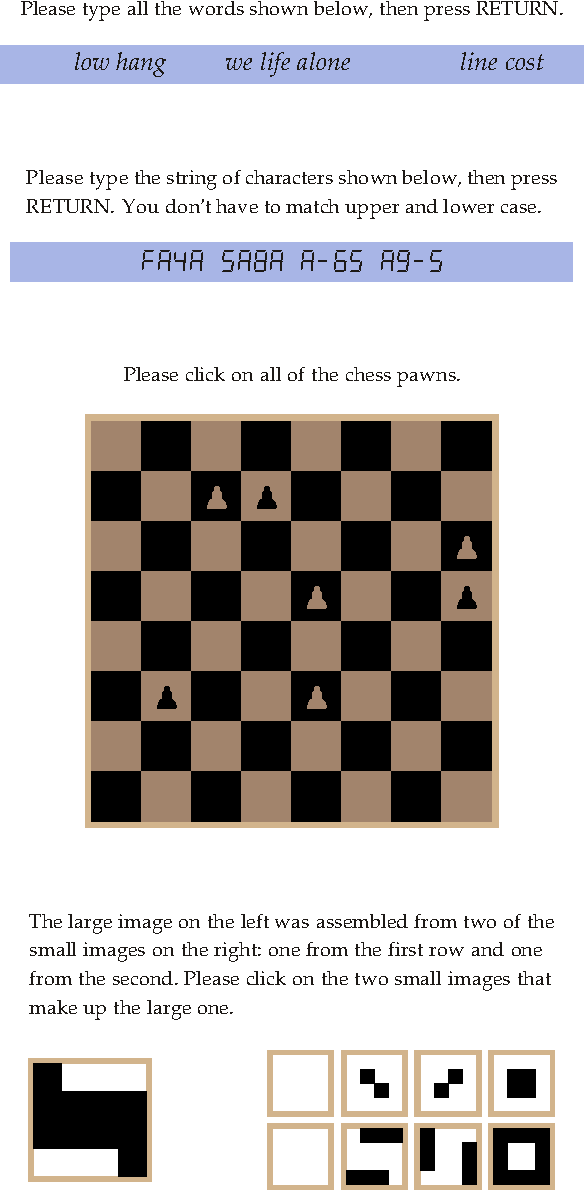
\includegraphics{tasks}}
\caption{Our four interactive tasks.  Top to bottom: word CAPTCHA,
  character CAPTCHA, chessboard, and visual matching.  Screen shots
  taken with Safari~4.0.}\label{fig:tasks}
\end{figure*}

All of our tasks operate within the constraints of Baron's defense:
they use visited-link styles only to change the color of text or
graphics on the screen.  They are designed to probe 8~to~100 links
each, which is small, but as demonstrated by Jang, not too small for
the sites currently making use of automated history exploits.
Finally, each task masquerades as an interaction that would not be out
of place on a honest website.  It is common for web sites to challenge
their visitors to perform a task that is relatively easy for a human,
but difficult for software~\cite{ahn03captcha}.  This is to prevent
automated abuse of a site (“spam” posts to a message board, for
instance).  Such challenges are referred to as
CAPTCHAs.\footnote{CAPTCHA is a contrived acronym for Completely
  Automated Public Turing test to tell Computers and Humans Apart.}
The most common type of CAPTCHA is a request to type either a few
words, or a string of random letters and numbers, from an image shown
on the screen.  The text is manipulated to defeat OCR software.
Another common type of CAPTCHA is a visual puzzle, to be solved using
the mouse; visual puzzles are also commonly presented as true games
(that is, intended only to entertain).

Interactive attacks necessarily involve placing hyperlinks on the
screen, and then inducing victims to do something with them that
will reveal to the attacker which ones are visited links.  Hyperlinks
have built-in interactive behavior that will reveal that something
fishy is going on, if a victim experiments with the page rather than
just following the instructions.  For instance, clicking on a link
(visible or not) will cause the browser to load the link destination;
hovering the mouse pointer over a link (again, visible or not) will
display the link's destination URL somewhere in the browser's “chrome”
(such as the status bar or the URL bar); selecting all the text on the
page will reveal text that has been hidden by drawing it with the same
color as the background.  Fortunately for the attacker, all these
inconvenient behaviors can be suppressed by positioning a transparent
image over all the hyperlinks.

Figure~\ref{fig:tasks} shows what each of our interactive attacks
looked like to a participant in the experiment, including the
instructions for each.  Note that we did not include the noise, lines,
or distortions typical of real CAPTCHAs; image recognition software
would have no trouble with any of them.  (If we had done this, the
tasks would also have been more difficult for our participants.)  An
attacker determined to make their phony CAPTCHAs look as much like
real ones as possible could use SVG transformations to distort the
text, and/or include lines and visual noise in the transparent image
superimposed on the links to suppress their normal behavior.

\subsubsection{Word CAPTCHA}

This is the simplest task.  Victims are asked to type several short
English words.  Each word is a hyperlink to an URL that the attacker
wishes to probe; if visited, the word is styled to be drawn in black
as usual, but if unvisited, it is drawn in the same color as the
background.  Thus, victims see only words corresponding to sites they
have visited.  The attacker must arrange for at least one word to be
visible no matter what; otherwise, a victim who has visited
\emph{none} of the URLs the attacker is probing will see a blank
CAPTCHA and think the site has malfunctioned.

This task is easy to perform, and simple to implement, but can only
probe a small number of links, since attackers cannot expect their
victims to be willing to type more than a few words.  In our study, we
used a maximum of ten words, of which one was always visible and one
always invisible; thus we could test no more than eight links.

\subsubsection{Character CAPTCHA}

\begin{figure}
\centerline{
\includegraphics[width=2in]{cc-exploded}}
\caption{7-segment LCD symbols stacked to test three links per
  composite character.  The \lcd{-} at the bottom is always visible,
  but the \lcd{4}, \lcd{5}, and \lcd{F} are only visible if a
  URL was visited.}\label{fig:sevenseg}
\end{figure}

This task is very similar to the previous one, but by clever choice of
font and symbols, it tests the visitedness of three links per
\emph{character} typed.  Victims are asked to type what appears to be
a string of letters, numbers, and dashes from a restricted character
set, in a font that mimics seven-segment LCD symbols.  As shown in
Figure~\ref{fig:sevenseg}, each visible character is actually \emph{four}
characters, superimposed, three of them visible only if an associated
link is visited.  No matter which combination of symbols is “on,”
their composite will always be a character that the victim can type,
and each combination produces a different composite. $\lcd{4} +
\lcd{5} = \lcd{9}$; $\lcd{4} + \lcd{F} = \lcd{A}$; $\lcd{5} + \lcd{F}
= \lcd{6}$; $\lcd{4} + \lcd{5} + \lcd{F} = \lcd{8}$.  The always-on
\lcd{-} is necessary because position within the overall string is
meaningful; without it, victims might see a series of blank spaces.
In response they would probably type only one space, and that would
make the result ambiguous.  Again, attackers cannot expect their
victims to type more than a few characters, but an eight-character
CAPTCHA of this design will probe~24 sites, and a 12-character one
will probe~36.

This attack has more technical complications to cope with than the
previous one.  Hardly anyone has a seven-segment LCD font installed,
but this is only a minor hurdle, as all modern browsers implement
site-supplied fonts~\cite{css3fonts}.  More seriously, Baron's
history-sniffing defense does not allow visited-link rules to change
the transparency of a color.  This restriction prevents timing attacks
(drawing partial transparency is slower than drawing opaque color) but
also makes it harder to compose characters by stacking them.
Attackers can work around this restriction by making the characters
\emph{always} be nearly (but not entirely) transparent, whether or not
they are visited links; this is allowed.  They are black if visited
and white if unvisited.  Each composite segment is thus drawn in a
shade of gray.  This might be acceptable; if not, attackers could
apply an SVG color transformation to map all shades of gray to solid
black.  Unfortunately, SVG is \emph{not} a universal
feature~\cite{svg_matrix}; IE did not support it at all before
version~9 (not yet released as of this writing) and no browser
implements the complete spec.

\subsubsection{Chessboard puzzle}

This task presents a chessboard grid (not necessarily the same size as
a standard chessboard) on the screen; some of the squares are occupied
by chess pawns.  Victims are asked to click on all of the pawns.  In
fact every square contains a pawn, but each is a hyperlink to a
different website, and only the pawns corresponding to visited sites
are made visible, using the same technique as for the word CAPTCHA;
invisible pawns are the same color as their background.  This is
technically straightforward; the only complication is that the pawns
must be rendered using text or SVG shapes, so their color can be
controlled from CSS.  Fortunately, Unicode defines dingbats for all
the standard chess pieces; in our implementation we used another
site-supplied font to ensure that participants got pawns rather than
“missing glyph” symbols.  An attacker might be able to rely on system
fonts for the pawn dingbat, but it's easy enough to use a site font
that there's no reason not to.

This puzzle is easy for victims to complete, and the grid can be at
least ten squares on a side---the only limits are the size of the
screen, and victims' patience---so this attack can test at least
100~links' visitedness.  However, it becomes tedious if there are more
than a few visible pawns.  Also, if used for a real attack, the page
would have no way to tell how many clicks each victim will make, so
attackers must resort to a time-out or an explicit “go on” button;
either might seem suspicious.

\subsubsection{Pattern matching puzzle}

In this task, victims are asked to select two images which, when
“assembled,” produce a composite image.  The composite is made up of
four SVG shapes, whose fill color depends on the visitedness of four
hyperlinks.  There are four choices for each of the two images to be
selected; together, they exhaust the sixteen possible appearances of
the composite image.  While this does rely on SVG, it only requires
basic drawing features that are universally supported (except by IE).

One encounter with this puzzle tests the visitedness of four links.
It could be presented as a brainteaser challenge, giving a malicious
site the opportunity to make each victim solve many instances of the
puzzle in succession, and so probe many links.  It is decidedly more
difficult than our other tasks, but it could be made easier by not
composing two images, or by adjusting the images to make the correct
answer more obvious.

\subsection{Procedure}

We constructed a website which would challenge participants to carry
out instances of each of the above four tasks.  We did not actually
sniff history in the implementation of these tasks, because our goal
was to prove that these tasks could be performed by a typical user
accurately, quickly, and without frustration.  If we had implemented
genuine history-sniffing attacks, we would not have known the ratio of
visited to unvisited links to expect for each prompt, nor would we
have been able to detect errors.  Instead, we randomly generated task
instances corresponding to known proportions of visited and unvisited
links. Each participant experienced a fixed number of trials of each
task, as indicated in Table~\ref{tbl:props}; each trial selected a
proportion uniformly at random without replacement from the
appropriate column of Table~\ref{tbl:props}.  The site automatically
skipped tasks that would not work with participants' browsers (notably
those that required SVG, for participants using IE).

\begin{table}
\caption{\mbox{Proportions of visited links used for each task.}
\mbox{$N =$ total number of links, $V =$ number of visited links.}}
\label{tbl:props}
\begin{center}
\def\IS{\hspace{7.5pt}}
\def\OS{\hspace{20pt}}
\def\H#1{\multicolumn{2}{c@{\OS}}{\hbox to0pt{\hss\textbf{#1}\hss}}}
\def\HE#1{\multicolumn{2}{c}{\hbox to0pt{\hss\textbf{#1}\hss}}}
\def\N{$N\!$}
\def\V{$V\!$}
\begin{tabular}{*{3}{r@{\IS}r@{\OS}}r@{\IS}r}
\toprule
\H{Word} & \H{Character} \\
\H{captcha}& \H{captcha} & \H{Chess} & \HE{Matching} \\
\H{9 trials}& \H{9 trials}& \H{12 trials}& \HE{12 trials} \\
\N&\V&\N&\V&\N&\V&\N&\V\\
\midrule
10 &  1 & 12 &  3 & 16 &  3 & 4 & 0 \\
10 &  1 & 12 &  6 & 16 &  3 & 4 & 0 \\
10 &  1 & 12 &  9 & 16 &  5 & 4 & 1 \\
10 &  2 & 24 &  6 & 16 &  5 & 4 & 1 \\
10 &  2 & 24 & 12 & 16 &  7 & 4 & 1 \\
10 &  3 & 24 & 18 & 16 &  7 & 4 & 1 \\
10 &  3 & 36 &  9 & 16 & 11 & 4 & 1 \\
10 &  3 & 36 & 18 & 16 & 11 & 4 & 1 \\
10 &  4 & 36 & 27 & 36 &  3 & 4 & 1 \\
10 &  4 & 48 & 12 & 36 &  3 & 4 & 1 \\
10 &  4 & 48 & 24 & 36 &  5 & 4 & 2 \\
10 &  4 & 48 & 36 & 36 &  5 & 4 & 2 \\
10 &  5 & 60 & 15 & 36 &  7 & 4 & 2 \\
10 &  5 & 60 & 30 & 36 &  7 & 4 & 2 \\
10 &  5 & 60 & 45 & 36 & 11 & 4 & 2 \\
10 &  6 &    &    & 64 &  3 & 4 & 2 \\
10 &  6 &    &    & 64 &  3 & 4 & 2 \\
10 &  6 &    &    & 64 &  5 & 4 & 2 \\
10 &  7 &    &    & 64 &  5 & 4 & 3 \\
10 &  7 &    &    & 64 &  7 & 4 & 3 \\
10 &  7 &    &    & 64 &  7 & 4 & 3 \\
10 &  8 &    &    & 64 & 11 & 4 & 3 \\
10 &  8 &    &    & 64 & 11 & 4 & 3 \\
10 &  8 &    &    &    &    & 4 & 3 \\
10 &  9 &    &    &    &    & 4 & 3 \\
10 &  9 &    &    &    &    & 4 & 3 \\
10 &  9 &    &    &    &    & 4 & 3 \\
   &    &    &    &    &    & 4 & 4 \\
   &    &    &    &    &    & 4 & 4 \\
\bottomrule
\end{tabular}
\end{center}
\end{table}

We recruited~307 participants from Amazon Mechanical Turk for a “user
study.”  Participants were required to be at least~18 years old, able
to see computer graphics and read English, and be using a browser with
JavaScript enabled.  The precise nature of the study was not revealed
until participants visited the site itself.  At that point they were
told:

\begin{quote}
We are studying how much information can be extracted from a browser's
history of visited web pages by interactive attacks---that is, attacks
that involve your doing something on a website that appears to be
innocuous. It used to be possible to probe your browsing history
without making you do anything, but browsers are now starting to block
those attacks, so interactive probes may become more common in the
future.

In this experiment you will carry out some tasks similar to the
ones that a malicious site might use to probe your browsing history.
These tasks do not actually probe your browsing history; instead we
measure how quickly and accurately you can do them. From this, we
will be able to infer how much information each of the tasks could
extract from your history.
\end{quote}

\noindent
All participants completed a consent form and then a short demographic
survey (reproduced in Appendix~\ref{sec:survey}), after which they
were given brief overall instructions:

\begin{quote}
This experiment is divided into several tasks.  To proceed to the
first task, click on its heading, which is right below these
instructions.  When you complete each task, the heading for the next
task will become selectable.
\end{quote}

\noindent
The tasks all included their own specific instructions, which are
reproduced in Figure~\ref{fig:tasks} above the facsimile of each task.
Each task also included a progress bar at the bottom of its screen
area (not shown in Figure~\ref{fig:tasks}) which indicated the number
of trials remaining for that task.  When participants reached the end
of a subtask, the page showed some graphs of their performance on that
task, as a reward (we do not show any of these graphs here, to avoid
confusion with our actual analysis).  At the very end of the
experiment, participants were thanked for their assistance and offered
an opportunity to see all of the data collected (in its raw form)
before sending it to our server.

The typing tasks gave no feedback until the end, but the clicking
tasks indicated errors immediately.  In the chessboard task, each pawn
turned green when clicked, but if a participant clicked on an empty
square, a red X would appear in that square.  In the matching task,
when a small image was clicked, its brown border would turn blue if
that was the correct choice, red if not.  In both cases, participants
had to produce the correct answers before the task would end.  A real
attack could respond to clicks in a similar fashion, but might not be
able to give exactly the same error feedback, because of the
limitations on visited-link styles imposed by Baron's defense.  For
instance, a version of the chessboard task that really sniffed history
could turn visible pawns green when clicked, and could cause red pawns
to appear in squares that had been empty before the click, but could
\emph{not} convert invisible pawns to visible Xes upon a click.

It was possible for participants to refuse to carry out the typing
tasks, by hitting the \textsc{return} key over and over again without
typing anything.  The matching task could also be skipped, via an
explicit “skip this task” button, because our implementation sometimes
malfunctioned and we were not able to isolate the bug, so we had to
give people a way to move on.  The chessboard task, however, could not
be skipped or refused.

For comparison purposes, we also ran three automated history-sniffing
exploits on all the participants.  Less than~13\% of the participants
were using a browser that blocked these exploits; see
Section~\ref{sec:demog} below for more on the experiment population.
We used \texttt{wtikay.com}'s set of 7012~commonly visited URLs
(derived from the Alexa top~5000~sites list~\cite{janc10wtikay,alexa})
for this test; we recorded only the total elapsed time and the number
of URLs detected as visited.

\subsection{Results}\label{sec:results}

\begin{figure}
\centerline{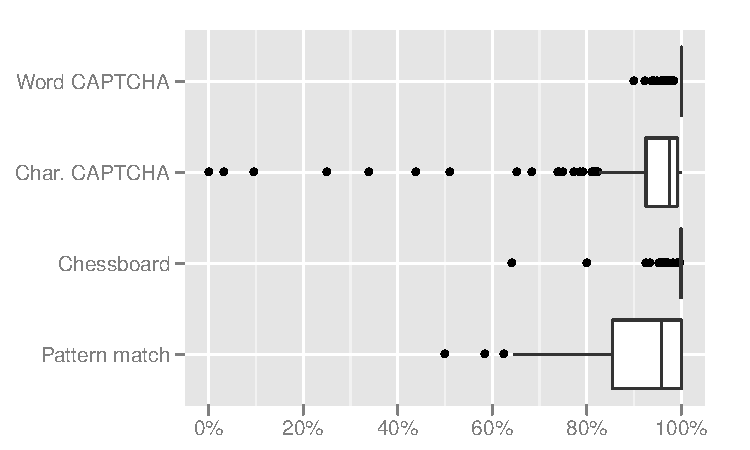
\includegraphics[width=3.5in]{accuracy}}
\caption{Overall accuracy rates for the four interactive
  tasks.}\label{fig:accuracy}
\end{figure}

\begin{figure}
\centerline{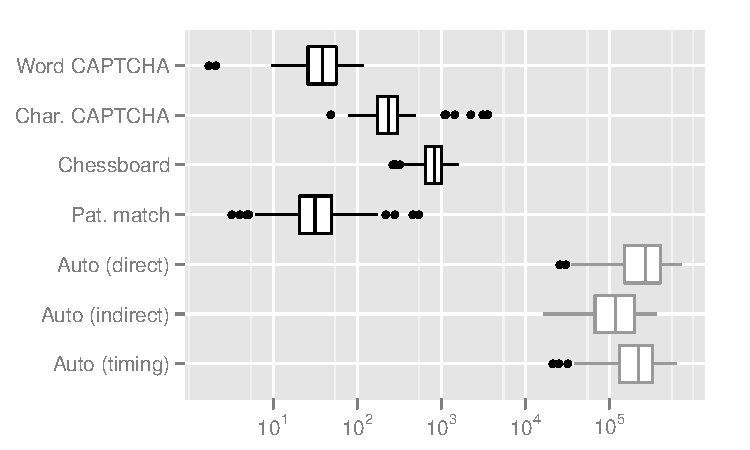
\includegraphics[width=3.5in]{qpm}}
\caption{Queries per minute achieved by the four interactive tasks
  (black) and three automated exploits (gray).}\label{fig:qpm}
\end{figure}

Not all of the participants completed all of the tasks successfully,
but we have usable data from at least 177~participants for each task.
Figure~\ref{fig:accuracy} shows raw user accuracy rate for all four
tasks.  The chessboard takes first place in accuracy, with nearly all
participants scoring~100\% or close to.  The word CAPTCHA is
substantially easier than the character CAPTCHA; the visual matching
task is dead last in terms of \emph{average} accuracy, but the
character CAPTCHA has a surprising number of outliers with very poor
accuracy.  We investigated these, and found that some participants
became so frustrated with the task that after a few trials they
started hitting \textsc{return} without attempting to type anything.
There are even a few~0\% scores, from participants who would not do
this task at all.  It is well known that strings of meaningless
characters are harder to type than strings of
words~\cite{hershman1965typing}, but we did not anticipate this level
of frustration.

Figure~\ref{fig:qpm} shows the achievable history-sniffing rate for
each task, with the rate of “traditional” automated attacks included
for comparison. Of the four interactive tasks, the chessboard puzzle
is the clear winner, achieving a median of nearly 1000~queries per
minute.  It should be remembered that this measurement combines two
factors: how fast a victim can do the task, and how many URLs the task
encodes.  The chessboard scores highly on both counts, but the
character CAPTCHA is only in second place because it encodes
many URLs.  Conversely, the word CAPTCHA is quick to complete,
but doesn't encode many URLs and therefore falls behind on QPM.
Matching does poorly on both factors.  And, unsurprisingly, all of our
interactive tasks are much slower than automated sniffing.

Since our study conditions are artificial, our participants'
performance (either speed or accuracy) does not translate directly to
attack effectiveness under “wild” conditions.  We challenged
participants to carry out dozens of instances of our tasks in quick
succession, whereas a real attack would require victims to complete
only one instance (except perhaps for the pattern-matching task).
However, we did not observe any significant effect of fatigue in our
tests, except for the participants who refused to complete all the
requested trials of the character CAPTCHA.  Some of the errors on the
typing tasks were caused by participants entering something completely
unexpected, rather than a possible but incorrect answer; in a real
attack, if this happened, the attacker would have to default to some
assumption about the links it was probing (most likely, that none of
them were visited) which might chance to be correct.  These effects
would tend to make a genuine attack more effective than our results
indicate.

On the other hand, our participants were told in advance that their
ability to carry out the tasks quickly and accurately was being
measured; people are known to perform better on tasks of this nature
when they know their performance is being tested (the “Hawthorne
effect”~\cite{hawthorne}).  Even if we had made the task conditions
mimic a real attack more precisely---perhaps we could have claimed
that we were evaluating the usability of new CAPTCHA styles---our
participants might have deduced that their performance was being
tested.  Furthermore, Mechanical Turk workers are paid for every task
they complete, so the faster they do tasks, the more money they earn;
our participant pool was therefore primed to carry out tasks as
quickly and accurately as they could before we ever started talking to
them.  These effects would tend to make a genuine attack \emph{less}
effective than our results indicate.  We should not discount the
motivation of victims faced with an (apparent) CAPTCHA, however.
CAPTCHAs are pure obstacles, so users are motivated to get them out of
the way as quickly as possible; users expect to be locked out of the
site if they fail to solve the challenge, so they are motivated to
solve them correctly.

On the whole, we think our results are a reasonable estimate of the
effectiveness of our tasks when used for a real sniffing exploit.
Attackers should perhaps worry more about CAPTCHAs causing some
fraction of their victims to abandon their efforts to use the
site~\cite{captcha-conversion}.  Even this can be addressed by making
the interactive task seem more like a game than an obstacle, and by
presenting it after potential victims have already sunk effort into
making use of the site.

\begin{figure}
\centerline{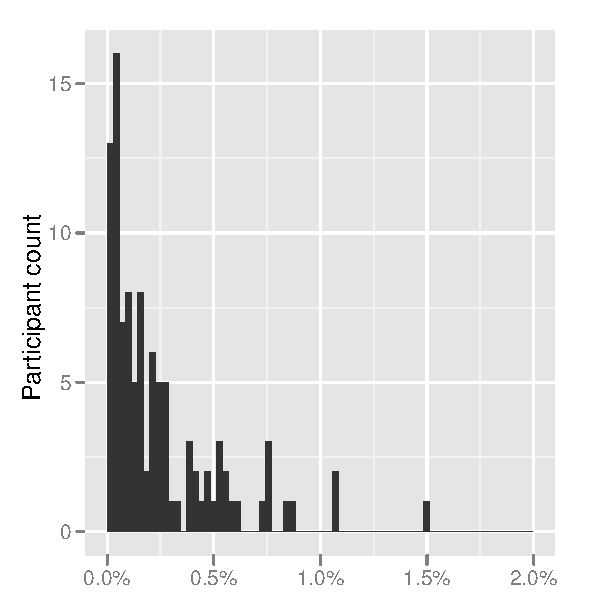
\includegraphics[width=3in]{visited-d}}
\caption{Histogram of percentage of links visited within
  \texttt{wtikay.com}'s set of 7012~commonly visited URLs (derived
  from the Alexa top 5000~sites), as measured by an automated history
  exploit.  No participant had visited more than a tiny fraction of
  these URLs.}
\label{fig:visited-density}
\end{figure}

\subsection{History Density}
The chessboard and word CAPTCHA are easier for the victim to
complete if they have visited only a few of the links that the
attacker is probing.  264~of our participants used a browser that
still permits automated history sniffing.
Figure~\ref{fig:visited-density} shows what percentage of the
\texttt{wtikay.com} “top5k” link set had been visited by each of them.
The percentages are clearly quite small, so attackers may be able to
assume a sparse set of visited links.  However, as pointed out by Janc
and Olejnik~\cite{janc10wtikay}, sparseness over this generic link set
may not equate to sparseness over a more targeted set---and the link
sets found by Jang were quite targeted indeed.

\subsection{Participant Demographics}\label{sec:demog}

\begin{figure*}
\centerline{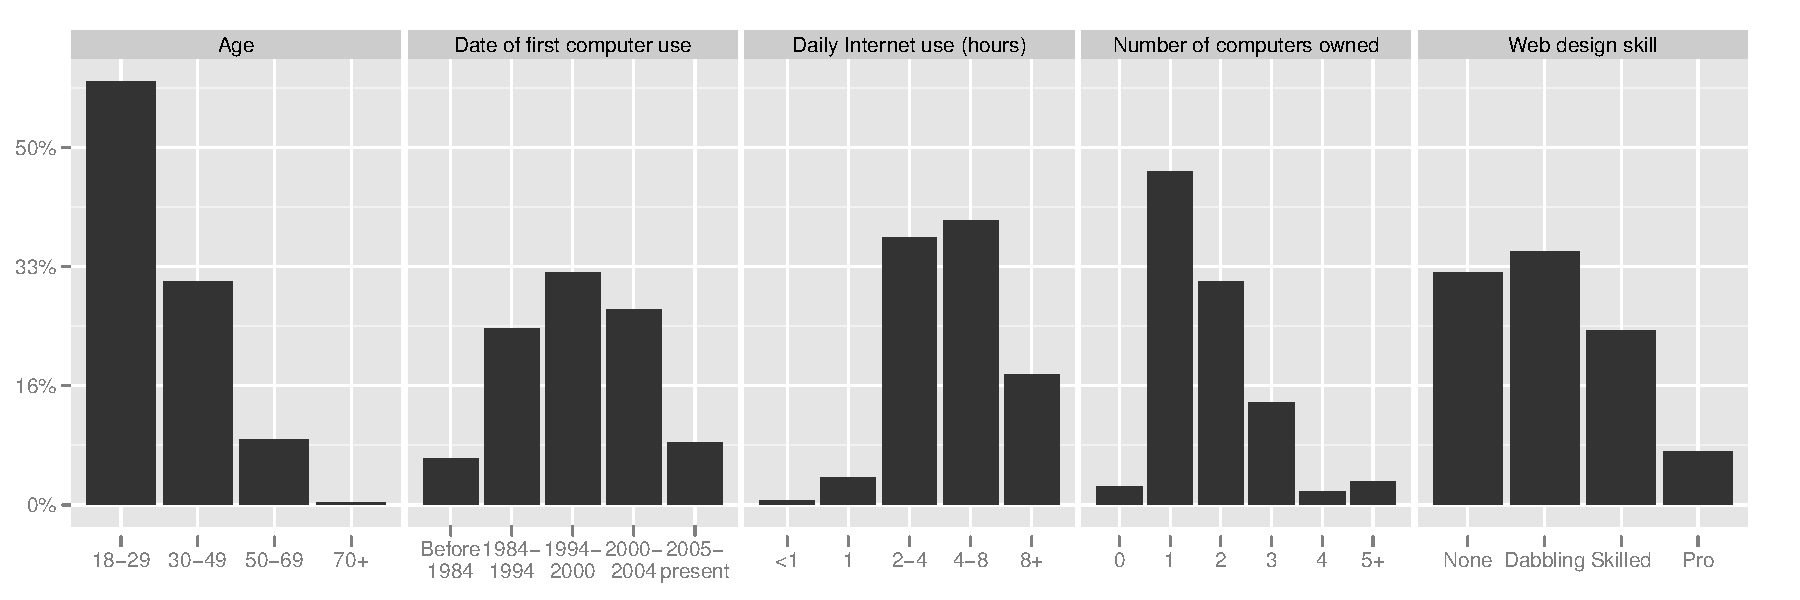
\includegraphics[width=7in]{demog}}
\caption{Demographic breakdown of participants}\label{fig:demographics}
\end{figure*}

We asked participants a few general questions about themselves; the
results are shown in Figure~\ref{fig:demographics}.  As the leftmost
graph in Figure~\ref{fig:demographics} shows, the study population is
strongly skewed to younger users, much more so than the (USA)
Internet-using population~\cite{pew_demog}.  Participants also appear
more likely than average to own more than one computer, use the
Internet frequently, have used computers for more than ten years
despite their youth, and to report having at least tried to put
together a website before.  This is consistent with other analyses of
the demographics of Mechanical Turk workers
specifically~\cite{mturk_demog,mturk_shift}.  We expect that our
conclusions about interactive tasks remain valid for Internet users at
large, since they rely mostly on measurements of basic motor
activities (typing, mousing).

\begin{figure}
\centerline{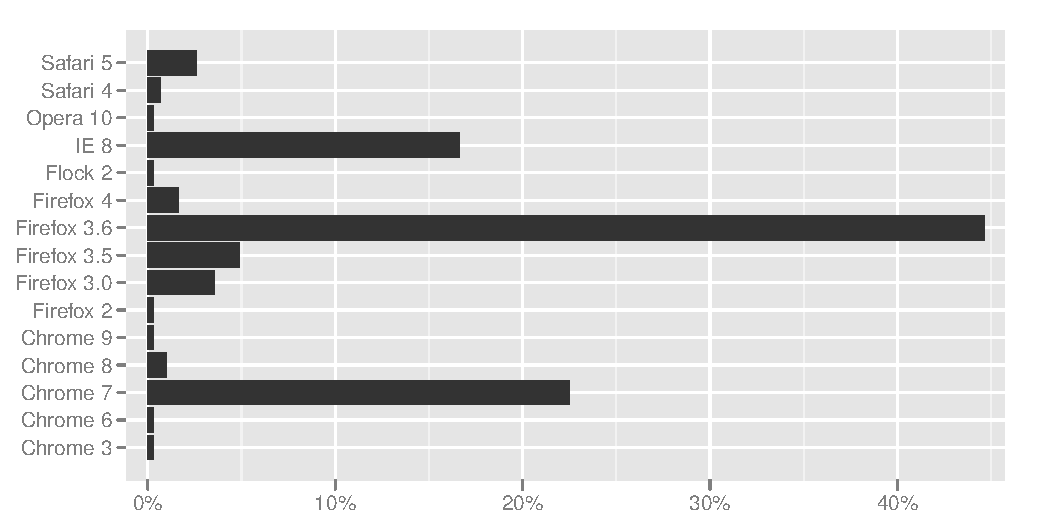
\includegraphics[width=3.5in]{browser}}
\caption{Browsers used by participants}\label{fig:browsers}
\end{figure}

Our participants used a wide variety of browsers, with the three most
popular being Firefox~3.6, Chrome~7, and IE~8.  Despite its place in
the top three, less than~20\% of participants used IE~8, and no older
versions of IE were detected; this also indicates a more technically
experienced population than the average.  The full breakdown is in
Figure~\ref{fig:browsers}.  We did not record participants' operating
systems, or any other User-Agent data beyond what is shown.  Safari~5,
Firefox~4, and Chrome~9 are the browsers that, at the time of the
study, implemented Baron's defense against automated history sniffing;
users of these browsers made up~13\% of our survey population.

\subsection{Discussion}\label{sec:discussion1}

We have shown that interactive attacks on visited-link history are
feasible, particularly if the attacker is interested only in a small
set of links, as were the real history sniffers found by Jang.
If we wish to defend against these attacks we must consider further
restricting the functionality of visited-link history---either the
circumstances under which links are revealed to be visited, or the
capabilities of visited-link styles.

Three of our four interactive attacks relied on making unvisited links
invisible by blending them into the background.  An obvious defense is
to prevent links from being drawn in the same color as the background
(whether visited or not).  However, merely determining what the
background color \emph{is} at any given position can be difficult.
Just to give one example, the attacker could make the background of
their fake CAPTCHA be partially transparent, then place a box of a
contrasting color directly underneath.  For efficiency, the browser
might prefer to have the computer's graphics card overlay the text,
the partially transparent background, and the colored box, and send
the result directly to the screen, but if it needs to know what the
color of the background plus the box is before it can draw the text,
it cannot do this.

But this is not the real problem with this defense.  The real problem
is that interactive attacks don't \emph{need} to make anything
invisible.  “Type the green words, but not the red words” would be an
even more convincing fake CAPTCHA than the one we used.  Similarly,
the chessboard task could ask the user to click only on red pawns.  As
long as there is a visible difference on the user's screen, we see no
practical way to prevent a sufficiently determined attacker from
getting the user to reveal what it is.

For the most privacy-conscious users, limiting the circumstances under
which visited links are revealed might be an appropriate move.  In his
original BUGTRAQ post describing visited link
attacks~\cite{bugtraq_visited}, Clover suggested that links might only
be revealed as visited when they refer to documents in the same domain
as the current page, but then immediately pointed out that this would
render the feature nearly useless.
SafeHistory~\cite{jackson06thirdpartycookies} refines this idea: links
are revealed as visited if they target a document in the same domain,
if the link destination has previously been visited from the current
site, or if the current site is on a whitelist of trusted sites.
Under this policy, a malicious site cannot learn anything from history
sniffing that it could not discover by monitoring clicks on outbound
links.  It sacrifices what is arguably the most useful case of
visited-link indications (when a new-to-the-user site links to a
document they have already seen), but to some extent this can be
mitigated by use of the whitelist.

Unfortunately, an attacker may still be able to construct an
interactive attack on history if \emph{any} links are revealed as
visited.  With SafeHistory in use, if attackers can predict the
location of a link to a site of interest on a whitelisted page, they
can draw pictures using \texttt{iframe}s that show one pixel of the
whitelisted page, directly above that link.  This is not so farfetched
as it might sound: a hyperlink to \texttt{facebook.com} appears at a
predictable location on the page
\url{http://www.google.com/search?q=facebook.com}, and search engines
are obvious candidates for whitelisting.  If there is no whitelist,
attackers could instead draw their pictures with single-pixel
\texttt{iframe}s of \emph{the sites they want to know about}.  Many
sites contain links pointing back to their front pages in predictable
locations on interior pages, which would count as same-origin and so
have their visitedness revealed.  (Care must be taken not to disturb
the visitedness of the front page, of course.)  Of course, attackers
using this technique cannot control the colors of visited and
unvisited links, but this poses little difficulty: they can either
design their interactive attack to work with the colors they get, or
they can use an SVG filter to remap the colors as they see fit (as we
did in the character CAPTCHA).

Most browsers can be configured not to retain any visited-link history
at all, and the “private browsing” mode found in all modern browsers
makes this quite convenient.  Private browsing was developed to defend
users' privacy against other users of the same
computer~\cite{private_browsing_paper}, but it also prevents remote
history sniffing attacks.  Of course, this comes at the price of not
distinguishing visited from unvisited links at all.  Alternatively,
most browsers can be configured to remember history only until shut
down; this mode's visited-link distinctions are less useful (the user
probably remembers what they have visited within the current session)
and remote attackers can still detect pages visited within the current
session.

\section{Experiment~2: side-channel attack}\label{sec:sideexpt}

Baron's defense \emph{was} intended to cover all practical side
channel attacks on browsing history; many of the restrictions it
places on \texttt{:visited} are solely to prevent timing attacks.
In Section~\ref{sec:sidechannel}, we described a practical side
channel attack on Firefox~4 beta using the \texttt{MozAfterPaint}
event. Unfortunately, this is not the only side channel attack for
history detection.  We discovered another attack that is technically
out of scope for the defense, as it relies on both software and
\emph{hardware} outside the browser's control, and would be difficult
to exploit in practice, but would also be very hard to close.

\subsection{Webcam attacks}

Many computers, especially laptops, nowadays come with a built-in
video camera aimed at the user.  Adobe Flash (not a standard component
of the Web, but very common nonetheless) includes a mechanism for
activating this camera and gaining direct access to the data stream it
produces.  Computer screens are backlit, so they illuminate the user
and the user's environment; the color of this light varies with the
color of the computer screen.  Thus, if the color of an area of the
screen depends on whether or not a link has been visited, an attacker
could use the camera to detect that color.  This attack will work
better if the colored area is large and the difference between the
visited and unvisited colors is dramatic, but in theory, sophisticated
image processing code could detect even small differences.

There are two major obstacles to this attack. First, the Flash runtime
will not activate the camera without the user's permission, and it
includes defenses against “clickjacking” attacks that trick the user
into granting permission~\cite{clickjacking,flash-clickjacking}.  The
attacker would have to make their site appear to have a legitimate use
for the camera; for instance, it could present itself as a video chat
site.  Second, to probe many links, it is necessary to change the
color of the link frequently---that is, to make some part of the
screen flash, which annoys users even in tiny doses, as the
\verb|<blink>| tag demonstrates.  If the color, size, or blink rate
are poorly chosen, flashing light can even induce epileptic
seizures~\cite{wcag}.  However, despite these drawbacks, many online
ads already do include blinking effects; an attack disguised as one of
these ads might irritate victims enough that they close the offending
window, but is unlikely to seem suspicious.

We developed and tested two variants of this attack.  In both
variants, we made a rectangular box of uniform color be a hyperlink,
periodically changed its target, and monitored changes in the average
color detected by the camera.  We used the least sophisticated image
processing algorithm that would work at all; our results should
therefore be considered a worst case scenario for the attacker.  The
QPM ratio and total number of links probed are fixed by the blink rate
and runtime of the attack, so we discuss only accuracy below.  As with
the interactive attacks, we did not actually sniff history; rather, we
generated a random sequence of 20~links, of which 10~were known to be
visited and 10~known to be unvisited, so that we knew the correct
answer for each link and could measure accuracy.

\subsubsection{Variant~1}
The first variant was designed to comply with the WCAG standard for
seizure safety~\cite{wcag}.  This standard limits the maximum area
that can be made to blink, maximum blink rate, and the maximum
luminosity difference between flashes; it also requires avoidance of
the color red.  All these requirements, especially the limits on
blinking area and luminosity changes, make detecting the change in
reflected light more difficult, but by no means impossible.

\subsubsection{Variant~2}
The second variant made the entire browser window flash, and used
brighter colors to represent visited and unvisited links.  The image
processing task is much easier, but it is obvious that something
unusual is happening.

\subsection{Results}
We tested both variants on ourselves under controlled conditions,
using one of the authors' computers (a Macbook Pro with built-in
webcam) in three settings with diverse backgrounds: an office cubicle,
a bedroom, and a living room.  We also tested the attacks both with
one of the authors sitting in front of the computer, and with nobody
in the camera's field of view.  We were able to achieve~100\% accuracy
for both variants in all conditions, provided that the room was
well-lit and the person in front of the computer (if any) remained
still.  In a dark room, accuracy dropped to chance~(50\%).

The first variant of the webcam attack was also field-tested as an
optional task for participants in our interactive experiment.  Not all
of them had Flash-accessible cameras or were willing to let us use
them; of the 307~participants in the interactive experiment, only~60
performed the webcam task.  Participants who agreed to perform the
task were asked to sit still and watch the screen while it flashed;
they did not need to do anything.

\begin{figure}
\centerline{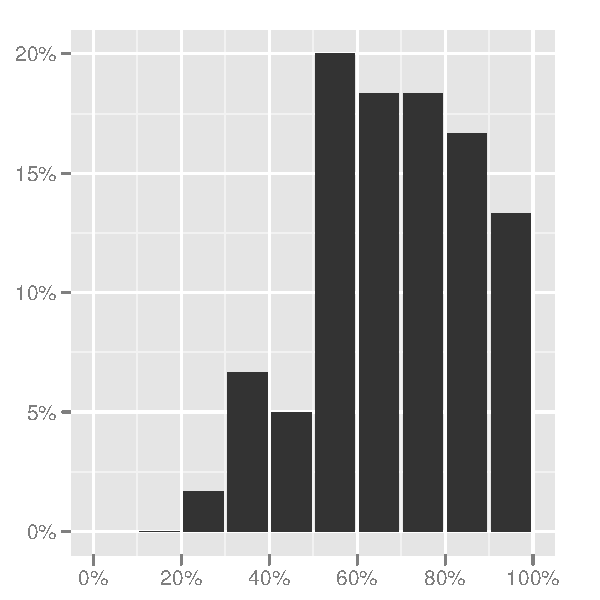
\includegraphics[width=3.5in]{webcam}}
\caption{Histogram of webcam attack (variant~1)'s accuracy rate when
  presented to participants in the interactive experiment.}
\label{fig:webcam}
\end{figure}

As shown in Figure~\ref{fig:webcam}, this attack's accuracy rate is
highly variable in the field, often dropping to not much better than
chance.  Comparing to our results under controlled conditions, we
believe the high error rate is mainly caused by participants moving
around during the task.  If so, attackers could analyze the video feed
and only run the attack during periods when nothing was moving in the
camera's field of view.  More sophisticated image processing might
also help.

\subsection{Discussion}

One might reasonably ask whether this technique is practical enough to
be a genuine threat.  We think the most serious obstacle in real life
would be persuading victims to allow access to their webcams.  There
are already sites that make legitimate use of the webcam, usually for
live two-way chat (the ChatRoulette service~\cite{chatroulette} is a
prominent example).  Such sites could plausibly incorporate the
WCAG-compliant variant of this attack, disguised as an ad.  The more
obtrusive variant is likely to make anyone who sees it close the
browser immediately, but we think it could still be used on victims
who walk away from the computer leaving the malicious site open.  It
does not take terribly sophisticated image processing to detect when
nobody is in the camera's field of view, and in our controlled tests,
the attack works even when the closest reflector is a wall 10~to~20
feet away from the monitor.

We would also like to point out that as the Web platform gains
capabilities, other side-channel attacks may become possible.  HTML5
already contemplates adding features~\cite{html5_device} that would
eliminate the need for Adobe Flash in the webcam attack.
WebGL~\cite{webgl} allows rendered HTML pages to be processed by
shader programs, which are Turing-complete; we speculate that they
might be able to detect history-dependent color changes and report
them back to the controlling page's scripts (if only via a timing
channel).

\section{Related Work}\label{sec:relatedwork}

Privacy attacks have received significant attention
recently. Section~\ref{sec:background} covered the existing work on
defenses for noninteractive attacks on visited-link
history~\cite{bugtraq_visited, moz_visited_bug, jang10empirical,
  jackson06thirdpartycookies, browserrecon, janc10wtikay,
  wondracek10deanon}. In this section, we describe related work on
privacy attacks that abuse other browser features.

Visited-link state is not the only way to determine whether the user
has visited a site.  Two other straightforward techniques involve
timing attacks on local caches maintained by the browser.

\begin{LaTeXdescription}
\item[Page cache.]
  Browsers cache resources retrieved from the Web to improve the speed
  of subsequent page loads. Approximately~60\% of HTTP queries are
  requests for cacheable resources~\cite{wolman99organization}.  The
  cache is global, so by embedding a resource from another site and
  measuring the time it takes to load, a web page can determine
  whether that resource is already in the browser's cache, and thus
  determine whether the user has visited the other
  site~\cite{felten00timing}.

\item[DNS cache.]  Name-to-IP-address mappings retrieved from the DNS
  are typically cached by the operating system of the computer that
  made the query, and may also be cached by an intermediate device
  (such as a network router) for the benefit of other computers on the
  same network.  Web attackers can induce the browser to perform a DNS
  lookup and measure the amount of time it
  takes~\cite{felten00timing}; local network attackers, able to make
  queries of a shared DNS cache, can inspect its contents in more
  detail~\cite{dnsprefetch,dnssnoop}.  The DNS cache can reveal which
  sites a user has visited, but unlike the page cache, it can also
  reveal search queries that the user has made, because some browsers
  (versions of Firefox and Chrome released since 2008~\cite{dnssnoop};
  Safari~5 also adopted the tactic) \emph{prefetch} DNS entries for
  sites that the user is likely to visit in the future---such as sites
  linked from a search results page.
\end{LaTeXdescription}

\noindent
Note that both these techniques are destructive---only the very first
attempt to determine whether a piece of information is cached will
reveal anything interesting, because the attack itself causes the
information to be cached.  Also, browsers don't cache information for
very long, even in the face of strenuous efforts by site maintainers
to make them do so~\cite{cachelife2007,cachelife2010} so these attacks
are not very reliable and may only reveal short-term history.

Another tactic only applies to sites that users typically remain
logged into for long periods (Facebook, Gmail, Twitter, etc.)  If an
attacker can guess the URL of a resource that is loadable cross-origin
but only available to logged-in users, they can attempt to load it and
detect failure using the JavaScript \verb|onerror| event.  Depending
on the site, more information may be available to clever
attackers~\cite{brewster08login}; even if the resource does not
generate an HTTP error for users that are not logged in, it may be
possible to extract information from it~\cite{thinkermade08focus}.

Client-side state such as cookies~\cite{httpstate_old,httpstate},
Flash Player local shared objects~\cite{lso}, and Web
Storage~\cite{webstorage} can be used by web sites to re-identify
users who have visited a site in the past.  They are often used for
user authentication and personalization.  Some of these mechanisms
(notably cookies) allow “third parties” (sites other than the main one
the user is interacting with, but that provide some of the resources
present in the page) to access client-side state.  This third-party
state is separate from any state set by the page itself, but if
several sites refer to the same resource provider (for instance, an
advertising network), that provider can build a profile of a user's
browsing activities.  Even if the user regularly clears their cookies,
a determined site may be able to re-construct them based on other
browser state~\cite{evercookie}.  Most browsers provide some degree of
control over cookies, allowing users to disable third-party cookies
altogether, or allow only cookies with an acceptable P3P privacy
policy~\cite{p3p}. Unfortunately, these mechanisms are easily
circumvented~\cite{jackson06thirdpartycookies,cranor-bad-p3p}.

Finally, many kinds of technological devices possess subtle but
measurable variations that allow them to be “fingerprinted,” and
browsers are no exception. By tracking information that the browser
reveals to all sites, such as \verb|User-Agent| headers, \verb|Accept|
headers, screen resolution, time zone, browser plugins, and system
fonts, a site can rapidly re-identify users, even without the use of
client-side state~\cite{pamphleteer,panopticlick}.  Fingerprinting can
be used to build a profile of user behavior even if the user tries to
clear browser state.

Privacy tools such as Torbutton~\cite{torbutton} aim to mitigate or
prevent the above attacks, at the cost of web functionality; this is
an acceptable tradeoff for some users.  Torbutton is particularly
noteworthy for considering and designing against fingerprintability.
Private browsing mode~\cite{private_browsing_paper} can also mitigate
some of these attacks, but it was not designed to do so and is less
effective than a specialized tool; again, functionality is sacrificed.
Ad-blockers~\cite{adblock} prevent many real-world cases of behavior
profiling as a side effect, since ad networks are one of the primary
users of third-party cookies.

The more well-known providers of third-party tracking cookies often
allow users to “opt out”~\cite{wpfoptout}, but this is a manual
procedure that must be carried out for each tracker.  The “Do Not
Track” initiative~\cite{donottrack} proposes to indicate in HTTP
request headers when users do not wish to be tracked; to be effective
this would have to be backed up with sanctions against tracking
agencies that ignore it, and at present there is no legal framework
for such sanctions.

\section{Conclusion}\label{sec:conclusion}

Web browsers attempt the difficult balancing act of preserving their
users' privacy and security, while simultaneously exposing as much of
their computers' capabilities as possible to untrusted code from the
Internet.  In this paper we examined an attack, history sniffing,
which appeared as an unintended consequence of the combination of
three independently desirable features: visited-link indication to the
user, CSS control of all aspects of page appearance, and JavaScript
monitoring of page rendering.  Automated history sniffing attacks,
including timing attacks, have successfully been blocked in the latest
browsers by David Baron's restrictions on visited link
styling~\cite{moz_visited_defense}.  However, attacks that involve the
user remain possible, as do attacks via side channels outside of the
browser's control.

We developed proofs of concept of six history sniffing exploits that
remain possible with Baron's defense in place: four involving
interaction with the user, and two involving detection of the color of
the screen with a webcam.  We tested our exploits on 307~users from
Amazon Mechanical Turk, and found that while they are slower than
automated attacks, and less convenient for an attacker, they are
practical for small numbers of URLs, in the same range as the “wild”
automated exploits found by Jang~et~al.~\cite{jang10empirical}.

All of our exploits, fundamentally, depend only on the browser having
revealed a distinction between visited and unvisited links on the
computer screen, plus some way for the page to read that information
back---via the victim's eyes and hands, or via a camera controllable
by the webpage.  As browsers continue to add capabilities to the Web
platform, it seems inevitable to us that further ways will appear for
malicious pages to discover what only the user should know.  Link
visitedness is not the only case where browsers try to combine
information from mutually distrusting sources into one
apparently-seamless “page,” and all those other cases are also
problematic for security~\cite{roc:distinguish,annevk:consistency}.
We consider finding more reliable ways to make these combinations,
without compromising user privacy or cross-site security, an open
research problem crucial to the future of the Web.

\section*{Acknowledgements}

% list is in alphabetical order by last name
We thank
Adam Barth,
Pamela Griffith,
Jeremiah Grossman,
Artur Janc,
Łukasz Olejnik,
Jesse Ruderman,
Eric Seidel,
Hovav Shacham,
Nathaniel Smith,
Venkat Venkatakrishnan,
Helen Wang,
and
Dara Weinberg
for their helpful suggestions and feedback.

This research was supported by Microsoft Research and
CyLab at Carnegie Mellon under
grant DAAD19-02-1-0389 from the Army Research Office. The views and
conclusions contained here are those of the authors and should not be
interpreted as necessarily representing the official policies or
endorsements, either express or implied, of Microsoft, ARO, CMU, or the
U.S.~Government or any of its agencies.

Data analysis was done in R~\cite{rlang} with the “ggplot2” graphics
package~\cite{rggplot2}.

\bibliographystyle{IEEEtran}
\bibliography{visited}

\appendices
\section{Demographic Survey}\label{sec:survey}

This is the demographic survey presented to participants in the
interactive experiment.  In the actual study, the response choices
shown for each question were presented with an HTML drop-down
selection widget.  Participants were required to answer all questions.

\begin{quote}
We'd like to know a little bit about you and your experience with
computers.

\textbf{Roughly how old are you?}
\begin{itemize}
\item 18--29
\item 30--49
\item 50--69
\item 70$+$
\end{itemize}

\textbf{When did you first use a computer?}
\begin{itemize}
\item Less than 5 years ago
\item 5 to 10 years ago
\item 10 to 15 years ago
\item Before Windows 95
\item Before the Macintosh
\end{itemize}

\textbf{How long do you spend on the Internet each day?}
\begin{itemize}
\item Barely at all
\item 1 hour
\item 2-4 hours
\item 4-8 hours
\item More than 8 hours
\end{itemize}

\textbf{How many computers do you own?}
\begin{itemize}
\item 0
\item 1
\item 2
\item 3
\item 4
\item More
\end{itemize}

\textbf{Do you know how to program computers or build websites?}
\begin{itemize}
\item No
\item I’ve tried it a few times
\item Yes
\item Yes, and I’ve done it for a living
\end{itemize}

\textbf{What kind of mouse are you using?}
\begin{itemize}
\item Regular mouse
\item Trackball
\item Touchpad
\item Eraser-head mouse
\item Other
\end{itemize}

\end{quote}

% shut up an annoying and verbose warning
\CLASSOPTIONconferencefalse
\end{document}
